\documentclass[letterpaper,journal]{IEEEtran}
% IEEE journal format, up to 10 pages.
\usepackage{amsmath,amssymb,amsfonts}
\usepackage{amsthm}
\usepackage{graphicx}
\usepackage{booktabs}
\usepackage{multirow}
\usepackage{xcolor}
\usepackage{algorithm}
\usepackage[noend]{algpseudocode}
\usepackage{tikz}
\usetikzlibrary{arrows.meta,positioning,fit,backgrounds,calc}
\usepackage[hidelinks]{hyperref}
\usepackage[capitalise,nameinlink]{cleveref}
\usepackage{url}

\DeclareMathOperator*{\argmax}{arg\,max}
\DeclareMathOperator*{\argmin}{arg\,min}
\newtheorem{proposition}{Proposition}
\crefname{proposition}{Prop.}{Props.}
\crefname{algorithm}{Alg.}{Algs.}
\crefname{section}{Sec.}{Secs.}
\crefname{table}{Table}{Tables}
\crefname{figure}{Fig.}{Figs.}

% Set to \realdatatrue to include the real-imagery (Despina / Apollo) evaluation subsection.
\newif\ifrealdata
\realdatafalse

\newcommand{\LoneHard}{46.6}
\newcommand{\LoneLam}{0.50}
\newcommand{\LoneRone}{59.9}
\newcommand{\LtenHard}{47.7}
\newcommand{\LtenLam}{0.50}
\newcommand{\LtenRone}{60.7}
\newcommand{\fgwVsLgHi}{+2.0}
\newcommand{\fgwVsLgLo}{-0.6}
\newcommand{\fgwVsLgMean}{+0.7}
\newcommand{\fgwVsUotHi}{+1.1}
\newcommand{\fgwVsUotLo}{-0.8}
\newcommand{\fgwVsUotMean}{+0.2}
\newcommand{\fixIllCzero}{85}
\newcommand{\fixIllDrop}{13.6}
\newcommand{\fixIllHard}{27.6}
\newcommand{\fixIllHardVal}{27.6}
\newcommand{\fixIllLam}{0.50}
\newcommand{\fixIllRone}{47.3}
\newcommand{\fullVsZs}{30.2}
\newcommand{\gainZsHi}{25.7}
\newcommand{\gainZsLo}{22.4}
\newcommand{\gainZsMean}{24.0}
\newcommand{\galCV}{6.4}
\newcommand{\galCfive}{55}
\newcommand{\galCfour}{60}
\newcommand{\galCone}{69}
\newcommand{\galCsix}{44}
\newcommand{\galCthree}{67}
\newcommand{\galCtwo}{44}
\newcommand{\galCzero}{79}
\newcommand{\galDust}{0.4}
\newcommand{\galFastHard}{47.3}
\newcommand{\galFastLam}{0.56}
\newcommand{\galFastRone}{60.3}
\newcommand{\galHard}{47.6}
\newcommand{\galLam}{0.50}
\newcommand{\galRfive}{87.3}
\newcommand{\galRfivesd}{0.5}
\newcommand{\galRone}{59.8}
\newcommand{\galRonesd}{0.8}
\newcommand{\galRonezero}{94.6}
\newcommand{\galRonezerosd}{0.2}
\newcommand{\galSzeroCzero}{80}
\newcommand{\galSzeroHard}{47.8}
\newcommand{\galSzeroRone}{60.8}
\newcommand{\galVsSalHi}{+1.3}
\newcommand{\galVsSalLo}{-0.5}
\newcommand{\galVsSalMean}{+0.4}
\newcommand{\gemCfive}{25}
\newcommand{\gemCfour}{30}
\newcommand{\gemCone}{35}
\newcommand{\gemCsix}{20}
\newcommand{\gemCthree}{35}
\newcommand{\gemCtwo}{20}
\newcommand{\gemCzero}{55}
\newcommand{\gemRfive}{64.7}
\newcommand{\gemRfivesd}{0.3}
\newcommand{\gemRone}{31.5}
\newcommand{\gemRonesd}{0.4}
\newcommand{\gemRonezero}{79.4}
\newcommand{\gemRonezerosd}{0.2}
\newcommand{\lamQuarterHard}{48.1}
\newcommand{\lamQuarterLam}{0.25}
\newcommand{\lamQuarterRone}{60.7}
\newcommand{\lamThreeqHard}{48.2}
\newcommand{\lamThreeqLam}{0.75}
\newcommand{\lamThreeqRone}{59.2}
\newcommand{\lamZeroHard}{48.4}
\newcommand{\lamZeroLam}{0.00}
\newcommand{\lamZeroRone}{59.9}
\newcommand{\mSixteenHard}{45.9}
\newcommand{\mSixteenLam}{0.51}
\newcommand{\mSixteenRone}{57.7}
\newcommand{\mThirtytwoHard}{47.9}
\newcommand{\mThirtytwoLam}{0.50}
\newcommand{\mThirtytwoRone}{61.1}
\newcommand{\msFgwGain}{6.3}
\newcommand{\msFgwGainsd}{0.8}
\newcommand{\msFgwRone}{66.1}
\newcommand{\msFgwRonesd}{0.1}
\newcommand{\msMnnGain}{5.2}
\newcommand{\msMnnGainsd}{0.6}
\newcommand{\msMnnRGain}{6.9}
\newcommand{\msMnnRGainsd}{0.4}
\newcommand{\msMnnRRone}{66.7}
\newcommand{\msMnnRRonesd}{0.5}
\newcommand{\msMnnRone}{65.1}
\newcommand{\msMnnRonesd}{0.8}
\newcommand{\noDustHard}{49.3}
\newcommand{\noDustLam}{0.50}
\newcommand{\noDustRone}{62.1}
\newcommand{\nvCfive}{48}
\newcommand{\nvCfour}{56}
\newcommand{\nvCone}{67}
\newcommand{\nvCsix}{46}
\newcommand{\nvCthree}{65}
\newcommand{\nvCtwo}{46}
\newcommand{\nvCzero}{79}
\newcommand{\nvRfive}{86.6}
\newcommand{\nvRfivesd}{0.4}
\newcommand{\nvRone}{58.2}
\newcommand{\nvRonesd}{0.7}
\newcommand{\nvRonezero}{94.6}
\newcommand{\nvRonezerosd}{0.2}
\newcommand{\rrFgwBeta}{1}
\newcommand{\rrFgwCfive}{61}
\newcommand{\rrFgwCfour}{70}
\newcommand{\rrFgwCone}{74}
\newcommand{\rrFgwCsix}{46}
\newcommand{\rrFgwCthree}{76}
\newcommand{\rrFgwCtwo}{49}
\newcommand{\rrFgwCzero}{85}
\newcommand{\rrFgwHard}{52.2}
\newcommand{\rrFgwKappa}{80}
\newcommand{\rrFgwLocRone}{59.8}
\newcommand{\rrFgwRBeta}{0.5}
\newcommand{\rrFgwRCfive}{58}
\newcommand{\rrFgwRCfour}{66}
\newcommand{\rrFgwRCone}{72}
\newcommand{\rrFgwRCsix}{44}
\newcommand{\rrFgwRCthree}{74}
\newcommand{\rrFgwRCtwo}{47}
\newcommand{\rrFgwRCzero}{85}
\newcommand{\rrFgwRHard}{49.5}
\newcommand{\rrFgwRKappa}{20}
\newcommand{\rrFgwRLocRone}{63.0}
\newcommand{\rrFgwRRfive}{88.7}
\newcommand{\rrFgwRRone}{63.8}
\newcommand{\rrFgwRfive}{90.1}
\newcommand{\rrFgwRone}{66.0}
\newcommand{\rrGainHi}{6.3}
\newcommand{\rrGainLo}{4.1}
\newcommand{\rrGainMean}{5.2}
\newcommand{\rrGlobRfive}{88.0}
\newcommand{\rrGlobRone}{60.8}
\newcommand{\rrLgBeta}{1}
\newcommand{\rrLgCfive}{53}
\newcommand{\rrLgCfour}{68}
\newcommand{\rrLgCone}{79}
\newcommand{\rrLgCsix}{45}
\newcommand{\rrLgCthree}{76}
\newcommand{\rrLgCtwo}{52}
\newcommand{\rrLgCzero}{84}
\newcommand{\rrLgHard}{50.1}
\newcommand{\rrLgKappa}{160}
\newcommand{\rrLgLocRone}{57.5}
\newcommand{\rrLgRBeta}{4}
\newcommand{\rrLgRCfive}{53}
\newcommand{\rrLgRCfour}{69}
\newcommand{\rrLgRCone}{82}
\newcommand{\rrLgRCsix}{45}
\newcommand{\rrLgRCthree}{76}
\newcommand{\rrLgRCtwo}{50}
\newcommand{\rrLgRCzero}{85}
\newcommand{\rrLgRHard}{49.0}
\newcommand{\rrLgRKappa}{640}
\newcommand{\rrLgRLocRone}{60.0}
\newcommand{\rrLgRRfive}{89.8}
\newcommand{\rrLgRRone}{65.7}
\newcommand{\rrLgRfive}{89.6}
\newcommand{\rrLgRone}{65.3}
\newcommand{\rrMnnBeta}{1}
\newcommand{\rrMnnCfive}{58}
\newcommand{\rrMnnCfour}{69}
\newcommand{\rrMnnCone}{80}
\newcommand{\rrMnnCsix}{47}
\newcommand{\rrMnnCthree}{74}
\newcommand{\rrMnnCtwo}{47}
\newcommand{\rrMnnCzero}{86}
\newcommand{\rrMnnHard}{50.9}
\newcommand{\rrMnnKappa}{80}
\newcommand{\rrMnnLocRone}{59.2}
\newcommand{\rrMnnRfive}{89.5}
\newcommand{\rrMnnRone}{66.0}
\newcommand{\rrUotBeta}{0.5}
\newcommand{\rrUotCfive}{60}
\newcommand{\rrUotCfour}{69}
\newcommand{\rrUotCone}{74}
\newcommand{\rrUotCsix}{47}
\newcommand{\rrUotCthree}{78}
\newcommand{\rrUotCtwo}{49}
\newcommand{\rrUotCzero}{84}
\newcommand{\rrUotHard}{51.9}
\newcommand{\rrUotKappa}{20}
\newcommand{\rrUotLocRone}{57.0}
\newcommand{\rrUotRfive}{90.4}
\newcommand{\rrUotRone}{65.8}
\newcommand{\salCV}{0.18}
\newcommand{\salCfive}{53}
\newcommand{\salCfour}{59}
\newcommand{\salCone}{68}
\newcommand{\salCsix}{47}
\newcommand{\salCthree}{65}
\newcommand{\salCtwo}{46}
\newcommand{\salCzero}{78}
\newcommand{\salDust}{83.3}
\newcommand{\salFixIllRone}{46.9}
\newcommand{\salRfive}{87.3}
\newcommand{\salRfivesd}{0.7}
\newcommand{\salRone}{59.4}
\newcommand{\salRonesd}{0.7}
\newcommand{\salRonezero}{94.8}
\newcommand{\salRonezerosd}{0.2}
\newcommand{\salSkyCorr}{0.63}
\newcommand{\tBackbone}{228}
\newcommand{\tFgw}{43}
\newcommand{\tFgwK}{427}
\newcommand{\tGal}{3.0}
\newcommand{\tGem}{2.9}
\newcommand{\tLg}{19}
\newcommand{\tLgK}{192}
\newcommand{\tNv}{1.8}
\newcommand{\tSal}{3.0}
\newcommand{\tSp}{140}
\newcommand{\tUot}{8.3}
\newcommand{\zsCosCfive}{10}
\newcommand{\zsCosCfour}{18}
\newcommand{\zsCosCone}{36}
\newcommand{\zsCosCsix}{14}
\newcommand{\zsCosCthree}{25}
\newcommand{\zsCosCtwo}{18}
\newcommand{\zsCosCzero}{67}
\newcommand{\zsCosRfive}{50.3}
\newcommand{\zsCosRone}{26.8}
\newcommand{\zsCosRonezero}{60.8}
\newcommand{\zsEigCfive}{16}
\newcommand{\zsEigCfour}{22}
\newcommand{\zsEigCone}{34}
\newcommand{\zsEigCsix}{17}
\newcommand{\zsEigCthree}{25}
\newcommand{\zsEigCtwo}{17}
\newcommand{\zsEigCzero}{65}
\newcommand{\zsEigRfive}{53.0}
\newcommand{\zsEigRone}{28.1}
\newcommand{\zsEigRonezero}{64.1}
\newcommand{\zsRRHard}{31.9}
\newcommand{\zsRRRfive}{72.4}
\newcommand{\zsRRRone}{51.1}
\newcommand{\zsSaladCfive}{25}
\newcommand{\zsSaladCfour}{36}
\newcommand{\zsSaladCone}{47}
\newcommand{\zsSaladCsix}{24}
\newcommand{\zsSaladCthree}{32}
\newcommand{\zsSaladCtwo}{21}
\newcommand{\zsSaladCzero}{66}
\newcommand{\zsSaladHard}{23.4}
\newcommand{\zsSaladRfive}{65.4}
\newcommand{\zsSaladRone}{35.8}
\newcommand{\zsSaladRonezero}{77.7}

\begin{document}

\title{Galatea: An Optimal Transport Framework for Merging Global and Local Descriptors in
Visual Place Recognition on Extraterrestrial Surfaces}

\author{Raunak Sarbajna and Christoph F. Eick%
\thanks{The authors are with the Department of Computer Science, University of Houston,
Houston, TX, USA.}}

\markboth{Preprint}{Sarbajna and Eick: Galatea}

\maketitle

\begin{abstract}
Visual place recognition (VPR) on the Moon has to cope with black shadows that move with the Sun,
statistically self-similar crater fields and strongly non-Lambertian regolith. We present
\emph{Galatea}, a framework that treats both stages of two-stage VPR as optimal transport (OT).
For global aggregation, a semi-relaxed unbalanced OT problem defines a one-parameter family of
token-to-cluster assignments that contains the NetVLAD ($\lambda=0$) and SALAD ($\lambda=1$)
assignments as end points and a learned $\lambda$ in between. We prove that its truncated Sinkhorn
iterations converge linearly at rate $\lambda$, characterise the dust-bin as a logistic gate, and
show that after intra-normalisation the descriptor sees the transport plan only through per-token
weights, which predicts when the choice of $\lambda$ can matter. For global--local fusion, a
training-free partial fused Gromov--Wasserstein matching scores both the appearance and the layout of
keypoints, and a saturating fusion rule provably overrides the global ranking only where the global
margin is small. On LunarSim-VPR, a physically motivated benchmark that renders the same query poses
under seven Sun conditions, terrestrial models fall from about $\zsSaladCzero\%$ to $\zsSaladHard\%$
Recall@1 under large Sun changes. With a frozen backbone, every value of $\lambda$ gives
$\approx\galRone\%$ (zero-shot: $\zsSaladRone\%$), as the theory predicts. Fine-tuning the last
backbone blocks adds $11$--$19$ points; within the OT family the assignments stay within about two points and a
learned $\lambda$ stays at its initial value, behaving like a fixed one, while NetVLAD-style residual
aggregation pulls ahead ($\ftNvRone\%$). Fusion adds
$2$--$7$ points for every stage-1 model and local matcher, because it keeps about half of the queries
that local evidence rescues while breaking few that the global ranking already had right; the full system
reaches $\msnvFgwRone\%$. Illumination-diverse training remains the largest single factor.
\end{abstract}

\begin{IEEEkeywords}
Localization, visual place recognition, space robotics, optimal transport, deep learning for visual perception.
\end{IEEEkeywords}


% ======================================================================
\section{Introduction}\label{sec:intro}
% ======================================================================
Surface missions to the Moon need to know where they are without GNSS. Wheel and visual
odometry~\cite{maimone2007mer} drift without bound, so a rover periodically needs an absolute fix
or a loop closure. One way to get it is to recognise that the current view shows a place that is
already in a reference set, either imagery from an earlier traverse or views rendered from orbital
digital elevation models (DEMs)~\cite{johnson2008trn,ceresoli2025optical}. This is
\emph{visual place recognition} (VPR), usually posed as image retrieval against a geo-tagged
database~\cite{lowry2015visual,schubert2023tutorial}.

Modern VPR systems reach high recall on street-level benchmarks by aggregating deep local
features into a compact global descriptor~\cite{arandjelovic2016netvlad,radenovic2019gem,berton2022cosplace,berton2023eigenplaces,izquierdo2024optimal},
optionally followed by local-feature re-ranking~\cite{hausler2021patch}. The lunar surface
removes almost every cue these systems rely on:
\begin{itemize}
\item \textbf{Illumination.} There is no atmosphere to scatter light, so shadows are black and
sharp. Over a lunar day the Sun's elevation and azimuth sweep through large ranges, and the
same place can look entirely different at two times (\cref{fig:conds}).
\item \textbf{Self-similarity.} Craters and boulders follow power-law size--frequency
distributions~\cite{neukum2001cratering,melosh1989impact}, so terrain is statistically repetitive
at every scale and individual features are weakly discriminative~\cite{torii2013visual}.
\item \textbf{Photometry.} Regolith is strongly non-Lambertian, with phase-dependent limb
darkening and an opposition surge~\cite{mcewen1991photometric,hapke2012theory}, which violates the
brightness-constancy assumptions built into terrestrial descriptors.
\item \textbf{Data.} There is no large, pose-annotated lunar VPR dataset to train on.
\end{itemize}

Two design questions follow. \emph{How should tokens be aggregated} when a large and variable part of
every image (black sky, featureless regolith, moving shadows) carries no place information? And
\emph{how should local evidence be used} when local features respond mostly to shadow edges that move
with the Sun? This paper answers both within one framework, \textbf{Galatea}, which casts each stage
of two-stage VPR as an optimal-transport (OT) problem. Global aggregation becomes an assignment of
tokens to clusters and a dust-bin; local verification becomes a transport between keypoint sets that
respects their layout; and the two are combined by a fusion rule whose behaviour can be stated
exactly. Treating the stages as OT problems makes their design choices explicit and analysable: the
framework contains the assignments of NetVLAD and SALAD as special cases, its theory predicts when the
choice between them matters, and our experiments test those predictions with a frozen and with a
fine-tuned backbone. Our contributions are:
\begin{enumerate}
\item \textbf{An OT family of aggregators} (\cref{sec:uot}). A semi-relaxed unbalanced OT problem
defines token-to-cluster assignments indexed by one scalar $\lambda\in[0,1]$ that recovers the NetVLAD
soft-assignment ($\lambda=0$) and the balanced Sinkhorn assignment of SALAD~\cite{izquierdo2024optimal}
($\lambda=1$) \emph{exactly}; Galatea can also learn $\lambda$. We prove linear convergence with rate
$\lambda$ for the truncated iterations, characterise the dust-bin as a logistic gate on cluster
affinity, and show that intra-normalised descriptors see the transport plan only through per-token
weights (\cref{prop:uot,prop:contraction,prop:dustbin,prop:colinv}).
\item \textbf{OT-based global--local fusion} (\cref{sec:fgw,sec:fusion}). A training-free partial
fused Gromov--Wasserstein (FGW) matcher scores both the appearance and the relative layout of keypoints
and is invariant to similarity transforms (\cref{prop:inv}). A saturating fusion rule combines it with
the global similarity and provably overturns the global ranking only where its margin is small
(\cref{prop:override}).
\item \textbf{LunarSim-VPR} (\cref{sec:bench})\footnote{Code and data: \url{https://github.com/RaunakDune/galatea-lunar-vpr}. Project website and interactive demo: \url{https://lunarsim.org}.}, an open, procedurally generated benchmark
with a physically motivated renderer (crater size--frequency statistics, lunar-Lambert photometry
with opposition surge, cast shadows from local and regional relief) whose protocol separates
viewpoint change from controlled changes in solar elevation and azimuth.
\item \textbf{A controlled study of what matters} (\cref{sec:exp,sec:discussion}). Under identical
training, with three seeds and paired-bootstrap confidence intervals, we evaluate terrestrial models
zero-shot, the whole assignment family with a frozen and a fine-tuned backbone, four local scorers with
and without fusion, and the effect of training illumination. We distil the results into design
guidelines for lunar VPR.
\end{enumerate}

The findings are not all in favour of the most flexible model. With a frozen backbone every value of
$\lambda$ performs alike, exactly as \cref{prop:colinv} predicts. With a fine-tuned backbone the
family spreads only slightly, a learned $\lambda$ is no better than fixing it at its initial value, and
residual NetVLAD aggregation, a different design axis, pulls ahead.
Fusion, in contrast, helps every stage-1 model, and how local and global evidence are combined matters
more than which local matcher is used.

% ======================================================================
\section{Related Work}\label{sec:related}
% ======================================================================
\paragraph*{Global descriptors for VPR}
VLAD~\cite{jegou2010vlad} and its trainable counterpart NetVLAD~\cite{arandjelovic2016netvlad}
softly assign local features to clusters and sum their residuals. GeM pooling~\cite{radenovic2019gem}
and classification-based training at scale (CosPlace~\cite{berton2022cosplace},
EigenPlaces~\cite{berton2023eigenplaces}) give strong compact descriptors. MixVPR~\cite{alibey2023mixvpr}
mixes feature maps with MLPs. AnyLoc~\cite{keetha2024anyloc} showed that unsupervised aggregation of
DINOv2~\cite{oquab2024dinov2} features generalises across domains, including aerial and underwater
imagery. SALAD~\cite{izquierdo2024optimal} recast NetVLAD's assignment as balanced entropic OT
with a dust-bin on top of a partially fine-tuned DINOv2 backbone. Our aggregator generalises SALAD
to unbalanced OT and contains NetVLAD's assignment as a limiting case.

\paragraph*{Re-ranking and matching}
Two-stage pipelines re-rank global candidates with local evidence, for example multi-scale patch
descriptors~\cite{hausler2021patch} or keypoint matching with geometric verification. Learned
matchers such as SuperGlue~\cite{sarlin2020superglue} and LightGlue~\cite{lindenberger2023lightglue}
solve (or approximate) an OT problem with dust-bins over attention-refined
SuperPoint~\cite{detone2018superpoint} features. They are trained on terrestrial imagery and assume
that the descriptors carry enough appearance information. Our re-ranker is training-free. It adds a
Gromov--Wasserstein structural term~\cite{memoli2011gromov,peyre2016gromov}, in the fused form of
\cite{vayer2019fgw} and with partial mass~\cite{chapel2020partial}, so that matches must preserve
relative keypoint geometry.

\paragraph*{Optimal transport}
Entropic regularisation and the Sinkhorn algorithm~\cite{cuturi2013sinkhorn,peyre2019computational}
made OT differentiable and fast. Unbalanced OT replaces hard marginal constraints with divergence
penalties and keeps Sinkhorn-like scaling algorithms~\cite{chizat2018scaling}. Gromov--Wasserstein
distances compare metric spaces through their internal distances~\cite{memoli2011gromov} and are
used for structured matching~\cite{vayer2019fgw}. We use OT in both roles: as a layer inside the
descriptor and as a training-free matcher between keypoint sets.

\paragraph*{Planetary localisation}
Rovers rely on visual odometry~\cite{maimone2007mer}, and landers on terrain-relative navigation
against orbital maps~\cite{johnson2008trn}. Synthetic optical images rendered from DTMs support lunar
navigation~\cite{ceresoli2025optical}. Our DESPINA~\cite{nelsonarcher2026despina} synthesises
photorealistic horizon views for a given location and heading with DEM-conditioned diffusion.
Lunar crater images have been retrieved with visual and depth features~\cite{lunarcomplexfeatures}.
Surface-level place recognition under controlled illumination change remains largely unstudied.

% ======================================================================
\section{Problem Formulation}\label{sec:problem}
% ======================================================================
Let $\mathcal{D}=\{(\mathbf{I}^{\mathrm{db}}_r,\mathbf{x}_r,\psi_r)\}_{r=1}^{N}$ be a database of
reference images with known planar position $\mathbf{x}_r\in\mathbb{R}^2$ and heading $\psi_r$, and let
$\mathbf{I}^{q}$ be a query image taken at an unknown pose $(\mathbf{x}^q,\psi^q)$, generally under a
different illumination. A database image is a \emph{true match} of the query if
$\|\mathbf{x}_r-\mathbf{x}^q\|_2<\rho$ and $|\psi_r-\psi^q|_{\circ}<\vartheta$, where
$|\cdot|_\circ$ is the wrapped angular difference (we use $\rho=10$\,m, $\vartheta=60^\circ$).
VPR is posed as retrieval~\cite{lowry2015visual,schubert2023tutorial}: an encoder
$\Phi$ maps every image to a unit-norm global descriptor and the database is ranked by
cosine similarity $s_g(q,r)=\langle\Phi(\mathbf{I}^q),\Phi(\mathbf{I}^{\mathrm{db}}_r)\rangle$.
A two-stage system additionally re-scores the top-$K$ candidates with a local score
$s_\ell(q,r)$ computed from keypoint correspondences. Performance is measured by
Recall@$k$, the fraction of queries with at least one true match among the top-$k$ results:
\begin{equation}
\mathrm{R@}k=\frac{1}{|\mathcal{Q}|}\sum_{q\in\mathcal{Q}}\mathbf{1}\big[\exists\, r\in\mathrm{top}_k(q):\ r \text{ is a true match of } q\big].
\label{eq:recall}
\end{equation}

% ======================================================================
\section{Method}\label{sec:method}
% ======================================================================
\Cref{fig:arch} gives an overview. Stage~1 aggregates the patch tokens of a vision transformer into
a global descriptor by solving a \emph{semi-relaxed unbalanced} optimal-transport (UOT) problem
between tokens and a set of learned clusters plus a dust-bin (\cref{sec:uot}). Stage~2 re-ranks the
$K$ best candidates with a \emph{partial fused Gromov--Wasserstein} (FGW) matching of
keypoints, which scores both what the keypoints look like and how they are arranged
(\cref{sec:fgw}). The final ranking fuses the global and local scores (\cref{sec:fusion}).

\subsection{Tokens, scores and the assignment problem}\label{sec:tokens}
A DINOv2 ViT-B/14 backbone~\cite{oquab2024dinov2} produces $n$ patch tokens
$\mathbf{t}_1,\dots,\mathbf{t}_n\in\mathbb{R}^{d}$ and a class token $\mathbf{t}_{n+1}$
($d=768$; $n=300$ for a $210\times280$ input). Following~\cite{izquierdo2024optimal}, two small
MLPs map each token to an assignment score vector
$\mathbf{s}_i=(s_{i1},\dots,s_{im})\in\mathbb{R}^m$ over $m$ clusters and to a reduced feature
$\mathbf{f}_i\in\mathbb{R}^{\ell}$:
\begin{equation}
\begin{aligned}
\mathbf{s}_i&=\mathbf{W}_{s_2}\,\sigma(\mathbf{W}_{s_1}\mathbf{t}_i+\mathbf{b}_{s_1})+\mathbf{b}_{s_2},\\
\mathbf{f}_i&=\mathbf{W}_{f_2}\,\sigma(\mathbf{W}_{f_1}\mathbf{t}_i+\mathbf{b}_{f_1})+\mathbf{b}_{f_2}.
\end{aligned}
\label{eq:mlps}
\end{equation}
Unlike NetVLAD~\cite{arandjelovic2016netvlad}, the score layer is randomly initialised (no
$k$-means centroids), so no geometric prior on the clusters is imposed. A learnable scalar $z$
scores every token against an extra \emph{dust-bin} column, giving the augmented score matrix
$\bar{\mathbf{S}}=[\mathbf{S}\,|\,z\mathbf{1}_n]\in\mathbb{R}^{n\times(m+1)}$. Each token carries
unit mass, $\mathbf{a}=\mathbf{1}_n$, and the clusters and dust-bin have nominal capacities
$\mathbf{b}=(\mathbf{1}_m^\top,\,n-m)^\top$ (this requires $n>m$). We write
$H(\mathbf{P})=-\sum_{ij}P_{ij}(\log P_{ij}-1)$ for the entropy and
$\mathrm{KL}(\mathbf{x}\|\mathbf{y})=\sum_j x_j\log(x_j/y_j)-x_j+y_j$.

\paragraph{Two known special cases}
NetVLAD distributes each token's mass independently over the clusters with a softmax,
$P_{ij}=\mathrm{softmax}_j(s_{ij}/\varepsilon)$. This constrains only the rows of $\mathbf{P}$
(feature$\to$cluster) and ignores how much mass each cluster receives
(cluster$\to$feature). SALAD~\cite{izquierdo2024optimal} constrains both marginals by solving the
balanced entropic OT problem~\cite{cuturi2013sinkhorn}
\begin{equation}
\mathbf{P}^{\mathrm{bal}}=\argmax_{\mathbf{P}\ge 0,\ \mathbf{P}\mathbf{1}=\mathbf{a},\ \mathbf{P}^\top\mathbf{1}=\mathbf{b}}
\ \langle\bar{\mathbf{S}},\mathbf{P}\rangle+\varepsilon H(\mathbf{P}).
\label{eq:balanced}
\end{equation}
At convergence, with $n=300$ and $m=64$, \eqref{eq:balanced} puts exactly one unit of mass into
every cluster and $n-m=236$ units ($79\%$ of all mass) into the dust-bin, regardless of image
content. A priori this is a questionable prior on the lunar surface, where the fraction of
uninformative tokens (black sky, featureless regolith, saturated slopes) varies widely with the
horizon position and the Sun elevation. In practice SALAD truncates Sinkhorn after $L=3$
iterations, which relaxes the constraint somewhat (\cref{sec:stage1}). The formulation below makes
the relaxation explicit and controllable.

\subsection{Galatea: semi-relaxed unbalanced OT assignment}\label{sec:uot}
We keep the token constraint hard (every token distributes exactly its unit mass) but replace
the cluster/dust-bin constraint with a KL penalty of strength $\tau>0$~\cite{chizat2018scaling}:
\begin{equation}
\mathbf{P}^{\tau}=\argmax_{\mathbf{P}\ge 0,\ \mathbf{P}\mathbf{1}_{m+1}=\mathbf{a}}
\ \langle\bar{\mathbf{S}},\mathbf{P}\rangle+\varepsilon H(\mathbf{P})-\tau\,\mathrm{KL}\big(\mathbf{P}^\top\mathbf{1}_n\,\big\|\,\mathbf{b}\big).
\label{eq:uot}
\end{equation}
Define $\lambda=\tau/(\tau+\varepsilon)\in(0,1)$ and the log-sum-exp
$\mathrm{LSE}_j(x_j)=\log\sum_j e^{x_j}$. Proofs of all propositions are given in the supplementary material.

\begin{proposition}[Structure, limits]\label{prop:uot}
Problem~\eqref{eq:uot} has a unique solution of the form
$P^{\tau}_{ij}=\exp\big((\bar S_{ij}+f_i+g_j)/\varepsilon\big)$, where the potentials
$(\mathbf{f},\mathbf{g})$ satisfy
\begin{align}
f_i &= \varepsilon\log a_i-\varepsilon\,\mathrm{LSE}_j\big((\bar S_{ij}+g_j)/\varepsilon\big),\label{eq:f}\\
g_j &= \lambda\big[\varepsilon\log b_j-\varepsilon\,\mathrm{LSE}_i\big((\bar S_{ij}+f_i)/\varepsilon\big)\big].\label{eq:g}
\end{align}
(i) As $\tau\to0$ ($\lambda\to0$), $\mathbf{g}\to\mathbf{0}$ and
$P^{\tau}_{ij}\to a_i\,\mathrm{softmax}_j(\bar S_{ij}/\varepsilon)$: the NetVLAD soft-assignment,
augmented with a dust-bin.
(ii) As $\tau\to\infty$ ($\lambda\to1$), \eqref{eq:f}--\eqref{eq:g} become the balanced Sinkhorn
fixed-point equations and $\mathbf{P}^{\tau}\to\mathbf{P}^{\mathrm{bal}}$ of \eqref{eq:balanced}.
\end{proposition}
Hence a single scalar $\lambda$ interpolates continuously between NetVLAD-style and
SALAD-style assignment. Galatea \emph{learns} $\lambda=\mathrm{sigmoid}(\theta)$ jointly with the
rest of the head. Alternating \eqref{eq:f} and \eqref{eq:g} gives \cref{alg:uot}, which is SALAD's
Sinkhorn loop with the cluster-side update multiplied by $\lambda$; it costs $O(Lnm)$.

\begin{proposition}[Linear convergence]\label{prop:contraction}
Let $\Phi$ map $\mathbf{g}$ to the value of \eqref{eq:g} after substituting $\mathbf{f}(\mathbf{g})$
from \eqref{eq:f}. Then $\|\Phi(\mathbf{g})-\Phi(\mathbf{g}')\|_\infty\le\lambda\|\mathbf{g}-\mathbf{g}'\|_\infty$.
For $\lambda<1$ the iterates of \cref{alg:uot} therefore converge linearly,
$\|\mathbf{g}^{(L)}-\mathbf{g}^\star\|_\infty\le\lambda^{L}\|\mathbf{g}^{(0)}-\mathbf{g}^\star\|_\infty$,
at a rate independent of $\varepsilon$, $n$ and $m$.
\end{proposition}
For the balanced case ($\lambda=1$) the same map is only non-expansive in $\|\cdot\|_\infty$. Its
convergence is usually proved in Hilbert's projective metric, with a rate that depends on
$\varepsilon$ and on the dynamic range of $\bar{\mathbf{S}}$~\cite{peyre2019computational}.
\Cref{prop:contraction} instead gives an explicit, data-independent rate for every $\lambda<1$.
Numerically the bound is tight: on random score matrices the measured error ratio between
successive iterations approaches $\lambda$. With learned values of $\lambda$ (\cref{sec:exp}), a
small fixed $L$ is therefore justified.

\begin{proposition}[Dust-bin gating]\label{prop:dustbin}
For every $\lambda\in[0,1]$, after any token-side update \eqref{eq:f} (in particular at the
output of \cref{alg:uot}), the fraction of token $i$'s mass sent to the dust-bin is
\begin{equation}
P_{i,m+1}=\mathrm{sigmoid}\!\Big(\tfrac{1}{\varepsilon}\big[z+g_{m+1}-\varepsilon\,\mathrm{LSE}_{j\le m}\big((s_{ij}+g_j)/\varepsilon\big)\big]\Big),
\label{eq:gate}
\end{equation}
which, for fixed potentials $\mathbf{g}$, is strictly decreasing in every cluster score $s_{ij}$ and increasing in $z$.
\end{proposition}
The dust-bin therefore acts as a learned soft gate on the token's \emph{soft-max cluster affinity}.
Tokens that resemble no cluster, such as sky, smooth regolith or noise, are suppressed before
aggregation. In the relaxed problem, the potential $g_{m+1}$, and with it the total discarded
mass, adapts to the image instead of being fixed at $n-m$.

The next result shows which part of the transport plan the descriptor actually sees. It explains
the empirical behaviour reported in \cref{sec:ablation}.

\begin{proposition}[Column-scale invariance]\label{prop:colinv}
Let the descriptor be built from $\mathbf{P}$ by \eqref{eq:agg} followed by per-cluster (intra-)
$\ell_2$-normalisation. Then $\Phi$ is invariant to $\mathbf{P}\mapsto\mathbf{P}\,\mathrm{diag}(\mathbf{c})$
for any $\mathbf{c}>0$. In particular, for any plan of the form of \cref{prop:uot}, $\Phi$ depends on the
cluster potentials $\mathbf{g}_{1:m}$ \emph{only through} the token weights
$w_i=e^{f_i/\varepsilon}=a_i\big/\sum_{j\le m+1}e^{(\bar S_{ij}+g_j)/\varepsilon}$:
\begin{equation}
\frac{\mathbf{V}_{j,:}}{\|\mathbf{V}_{j,:}\|}=\frac{\sum_i w_i e^{s_{ij}/\varepsilon}\mathbf{f}_i}{\big\|\sum_i w_i e^{s_{ij}/\varepsilon}\mathbf{f}_i\big\|}.
\label{eq:colinv}
\end{equation}
\end{proposition}
Balanced and unbalanced assignments therefore differ only in how they \emph{weight tokens}, through
$w_i$. How much total mass each cluster receives is removed by intra-normalisation. Equation~\eqref{eq:colinv}
also shows that NetVLAD with a dust-bin ($\lambda=0$) is SALAD-style aggregation with the simplest
weights, $w_i=1/(\sum_{j}e^{s_{ij}/\varepsilon}+e^{z/\varepsilon})$.

\begin{algorithm}[t]
\caption{$\lambda$-scaled log-domain Sinkhorn (Galatea assignment)}\label{alg:uot}
\begin{algorithmic}[1]
\Require scores $\bar{\mathbf{S}}\in\mathbb{R}^{n\times(m+1)}$, marginals $\mathbf{a},\mathbf{b}$, $\lambda\in[0,1]$, iterations $L$
\State $\mathbf{f}\gets\mathbf{0}_n,\ \mathbf{g}\gets\mathbf{0}_{m+1}$ \Comment{$\varepsilon$ absorbed in $\bar{\mathbf{S}}$}
\For{$\ell=1,\dots,L$}
  \State $g_j\gets\lambda\,[\log b_j-\mathrm{LSE}_i(\bar S_{ij}+f_i)]$ \Comment{clusters + dust-bin (relaxed)}
  \State $f_i\gets\log a_i-\mathrm{LSE}_j(\bar S_{ij}+g_j)$ \Comment{tokens (hard)}
\EndFor
\State \Return $\mathbf{P}=\exp(\bar{\mathbf{S}}+\mathbf{f}\mathbf{1}^\top+\mathbf{1}\mathbf{g}^\top)$ with the dust-bin column removed
\end{algorithmic}
\end{algorithm}

\subsection{Aggregation and training}\label{sec:agg}
With $\mathbf{P}\in\mathbb{R}^{n\times m}$ (the dust-bin column dropped), the aggregated
descriptor is the matrix $\mathbf{V}\in\mathbb{R}^{m\times\ell}$ with entries
\begin{equation}
V_{j,k}=\sum_{i=1}^{n}P_{i,j}\,f_{i,k},\qquad j=1,\dots,m,\ \ k=1,\dots,\ell .
\label{eq:agg}
\end{equation}
As in~\cite{izquierdo2024optimal}, centroids are not subtracted. A scene descriptor
$\mathbf{g}_{\mathrm{sc}}=\mathbf{W}_{g_2}\sigma(\mathbf{W}_{g_1}\mathbf{t}_{n+1}+\mathbf{b}_{g_1})+\mathbf{b}_{g_2}$
summarises the class token. Each row of $\mathbf{V}$ is $\ell_2$-normalised (intra-normalisation),
$\mathbf{g}_{\mathrm{sc}}$ is $\ell_2$-normalised, and the concatenation
$[\mathbf{g}_{\mathrm{sc}};\mathrm{vec}(\mathbf{V})]$ is $\ell_2$-normalised again to give
$\Phi(\mathbf{I})\in\mathbb{R}^{256+m\ell}$ ($8448$-D for $m=64,\ell=128$).
We train with the multi-similarity loss and miner~\cite{wang2019ms} on batches of $P$ places
$\times$ $4$ views. Images of \emph{different} places closer than $15$\,m are masked out of the
negative set, because adjacent places along a traverse overlap visually.

\subsection{Stage 2: partial fused Gromov--Wasserstein re-ranking}\label{sec:fgw}
Repetitive crater and boulder fields make individual local descriptors ambiguous: two places may
share many similar-looking craters. What distinguishes them is \emph{where} those craters lie
relative to one another~\cite{torii2013visual}. Let $\{(\mathbf{u}_i,\mathbf{d}_i)\}_{i=1}^{p}$
and $\{(\mathbf{v}_k,\mathbf{e}_k)\}_{k=1}^{p'}$ be SuperPoint keypoints~\cite{detone2018superpoint}
(pixel positions and unit descriptors) of the query and a candidate. We define the appearance cost
$M_{ik}=1-\langle\mathbf{d}_i,\mathbf{e}_k\rangle$ and scale-normalised intra-image distance matrices
$C^{q}_{ii'}=\|\mathbf{u}_i-\mathbf{u}_{i'}\|/\mu_q$ and $C^{c}_{kk'}=\|\mathbf{v}_k-\mathbf{v}_{k'}\|/\mu_c$,
where $\mu$ is the mean pairwise distance in each image. The partial FGW
problem~\cite{vayer2019fgw,chapel2020partial} trades appearance against preservation of the
keypoint geometry:
\begin{multline}
\min_{\mathbf{T}\in\bar{\mathcal{U}}}\ (1-\alpha)\langle\mathbf{M},\mathbf{T}\rangle\\
+\alpha\!\!\sum_{i,i',k,k'}\!\!\big(C^{q}_{ii'}-C^{c}_{kk'}\big)^2T_{ik}T_{i'k'}
-\varepsilon_\ell H(\bar{\mathbf{T}}),
\label{eq:fgw}
\end{multline}
where $\bar{\mathbf{T}}\in\mathbb{R}^{(p+1)\times(p'+1)}$ augments $\mathbf{T}$ with dust-bins that
absorb non-co-visible keypoints~\cite{sarlin2020superglue}, and $\bar{\mathcal{U}}$ fixes unit mass per
keypoint, with $p'$ and $p$ units for the bins. We minimise \eqref{eq:fgw} by entropic mirror
descent~\cite{peyre2016gromov}. Each step linearises the quadratic term at the current transported
part $\mathbf{T}^{(r)}$ (normalised to unit mass, with marginals $\boldsymbol{\pi},\boldsymbol{\pi}'$):
\begin{equation}
\mathbf{G}^{(r)}=(\mathbf{C}^{q})^{\odot2}\boldsymbol{\pi}\mathbf{1}^\top+\mathbf{1}\boldsymbol{\pi}'^\top(\mathbf{C}^{c})^{\odot2}-2\,\mathbf{C}^{q}\mathbf{T}^{(r)}\mathbf{C}^{c\top}.
\label{eq:gwgrad}
\end{equation}
(this is the gradient of the quadratic term up to a factor $2$, absorbed into $\alpha$). It then solves an entropic OT problem with dust-bins on the fused cost
$(1-\alpha)\mathbf{M}+\alpha\mathbf{G}^{(r)}$ with the log-domain Sinkhorn algorithm. The initial plan
uses $\mathbf{M}$ alone. Correspondences are mutual arg-maxima of $\mathbf{T}$ with confidence
above $0.2$. They are verified with a MAGSAC++~\cite{barath2020magsac} fundamental-matrix
fit, and the local score $s_\ell$ is the number of inliers.

\begin{proposition}[Invariances of the structural term]\label{prop:inv}
The objective \eqref{eq:fgw}, and hence $s_\ell$ before geometric verification, is invariant to
any similarity transformation (rotation, translation, isotropic scaling) applied to the keypoint
positions of either image, and to any permutation of the keypoints.
\end{proposition}
Unlike homography- or epipolar-based scoring, the structural term thus needs no camera model.
It rewards candidates in which matched keypoints keep their \emph{relative} layout, which is
exactly the cue that separates two crater fields with similar statistics.

\subsection{Fusing global and local evidence}\label{sec:fusion}
The final score of candidate $r$ for query $q$ is
\begin{equation}
s(q,r)=s_g(q,r)+\beta\,\frac{s_\ell(q,r)}{s_\ell(q,r)+\kappa},
\label{eq:fusion}
\end{equation}
where the saturating map keeps one very textured candidate from dominating. $\beta$ and $\kappa$
are selected on the validation terrain. With $\beta\to\infty$ the method reduces to pure local
re-ranking, and with $\beta=0$ to the global ranking.

\subsection{Complexity}\label{sec:complexity}
\Cref{alg:uot} costs $O(Lnm)$ (about $6\cdot10^{4}$ operations for $L=3$), which is negligible
next to the ViT forward pass. Each FGW step costs $O(p^2p'+pp'^2)$ for \eqref{eq:gwgrad} plus
$O(p\,p')$ per Sinkhorn iteration. Re-ranking $K$ candidates with $R$ outer steps therefore costs
$O(KR\,p^3)$ for $p\approx p'$. Measured run times are reported in \cref{sec:runtime}.

\begin{figure*}[t]
\centering
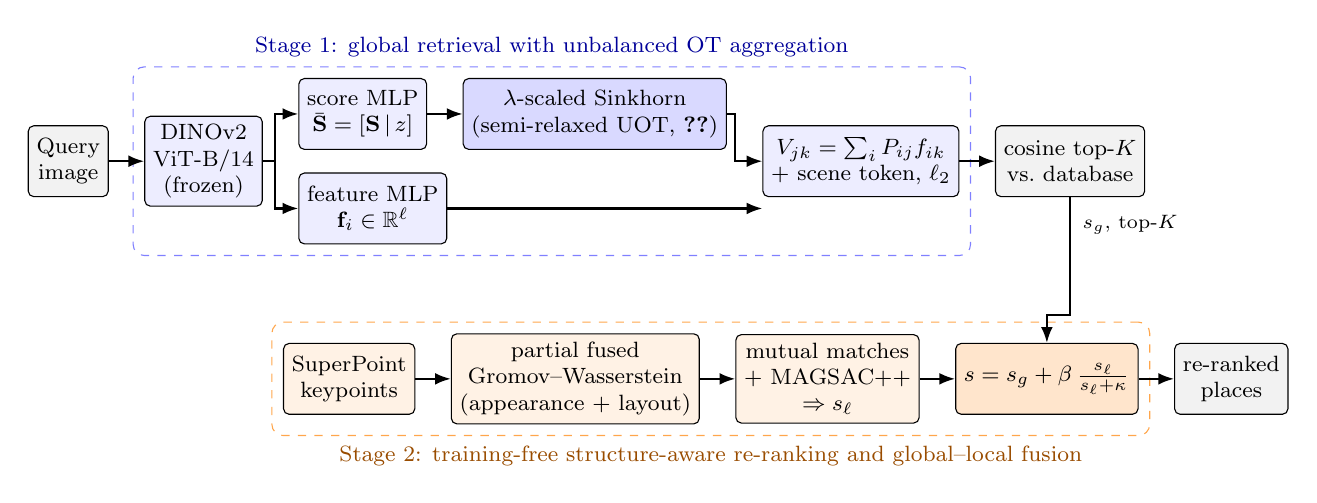
\begin{tikzpicture}[
  font=\footnotesize,
  box/.style={draw, rounded corners=2pt, align=center, minimum height=0.9cm, inner sep=3pt},
  st1/.style={box, fill=blue!7},
  st2/.style={box, fill=orange!10},
  io/.style={box, fill=gray!10},
  ar/.style={-{Latex[length=2mm]}, thick},
]
% stage 1
\node[io] (img) {Query\\image};
\node[st1, right=0.45cm of img] (vit) {DINOv2\\ViT-B/14\\(frozen)};
\node[st1, right=0.45cm of vit, yshift=0.6cm] (score) {score MLP\\$\bar{\mathbf S}=[\mathbf S\,|\,z]$};
\node[st1, right=0.45cm of vit, yshift=-0.6cm] (feat) {feature MLP\\$\mathbf f_i\in\mathbb R^{\ell}$};
\node[st1, right=0.45cm of score, fill=blue!15] (uot) {$\lambda$-scaled Sinkhorn\\(semi-relaxed UOT, \cref{alg:uot})};
\node[st1, right=0.45cm of uot, yshift=-0.6cm] (agg) {$V_{jk}=\sum_i P_{ij}f_{ik}$\\$+$ scene token, $\ell_2$};
\node[io, right=0.45cm of agg] (db) {cosine top-$K$\\vs.\ database};
\draw[ar] (img) -- (vit);
\draw[ar] (vit.east) -- ++(0.15,0) |- (score.west);
\draw[ar] (vit.east) -- ++(0.15,0) |- (feat.west);
\draw[ar] (score) -- (uot);
\draw[ar] (uot.east) -- ++(0.1,0) |- (agg.west);
\draw[ar] (feat.east) -- (agg.west |- feat.east);
\draw[ar] (agg) -- (db);
\begin{scope}[on background layer]
\node[draw=blue!50, dashed, rounded corners, fit=(vit)(score)(feat)(uot)(agg), inner sep=4pt,
  label={[blue!60!black]above:Stage 1: global retrieval with unbalanced OT aggregation}] {};
\end{scope}
% stage 2
\node[st2, below=1.25cm of feat, xshift=-0.3cm] (sp) {SuperPoint\\keypoints};
\node[st2, right=0.45cm of sp] (fgw) {partial fused\\Gromov--Wasserstein\\(appearance $+$ layout)};
\node[st2, right=0.45cm of fgw] (ver) {mutual matches\\$+$ MAGSAC++\\$\Rightarrow s_\ell$};
\node[st2, right=0.45cm of ver, fill=orange!20] (fuse) {$s=s_g+\beta\,\frac{s_\ell}{s_\ell+\kappa}$};
\node[io, right=0.45cm of fuse] (out) {re-ranked\\places};
\draw[ar] (db.south) |- ($(fuse.north)+(0,0.35)$) -- (fuse.north);
\node[font=\scriptsize, right=1pt] at ($(db.south)+(0,-0.35)$) {$s_g$, top-$K$};
\draw[ar] (sp) -- (fgw); \draw[ar] (fgw) -- (ver); \draw[ar] (ver) -- (fuse); \draw[ar] (fuse) -- (out);
\begin{scope}[on background layer]
\node[draw=orange!70, dashed, rounded corners, fit=(sp)(fgw)(ver)(fuse), inner sep=4pt,
  label={[orange!60!black]below:Stage 2: training-free structure-aware re-ranking and global--local fusion}] {};
\end{scope}
\end{tikzpicture}
\caption{Galatea. Stage~1 assigns ViT tokens to $m$ clusters and a dust-bin by semi-relaxed
unbalanced OT with a learned relaxation $\lambda$ ($\lambda{=}0$: NetVLAD assignment,
$\lambda{=}1$: SALAD), then aggregates them into a global descriptor. Stage~2 re-scores the top-$K$
candidates with a partial fused Gromov--Wasserstein matching of keypoints and fuses local and
global scores.}
\label{fig:arch}
\end{figure*}

% ======================================================================
\section{The LunarSim-VPR Benchmark}\label{sec:bench}
% ======================================================================
No public lunar surface dataset combines dense pose ground truth with systematic illumination
coverage. We therefore built a lightweight, reproducible renderer that targets the three properties
that make lunar VPR hard: self-similar relief, hard shadows and non-Lambertian photometry. It does
not replace real data (\cref{sec:limits}), but it lets us vary one factor at a time with exact
ground truth. It complements DESPINA~\cite{nelsonarcher2026despina}, which produces realistic
appearance for real sites from LRO DEMs but does not expose explicit control of the Sun direction.

\paragraph*{Terrain}
Each scene combines a \emph{regional} DEM ($16$\,m/px, $16.4$\,km) and a \emph{local} DEM
($0.3$\,m/px, $614$\,m) blended into its centre. Both start from fractional-Brownian relief
(power spectrum $\propto k^{-\beta}$, $\beta\in[2.2,3.2]$). Craters are drawn from an
equilibrium-like cumulative size--frequency distribution $N(>D)=cD^{-2}$~\cite{melosh1989impact}
($D\in[60,2500]$\,m regionally and $[1.5,120]$\,m locally) and stamped with a bowl--rim--ejecta
profile whose depth-to-diameter ratio ($0.04$--$0.2$) and rim height depend on a random degradation
state. Fresh craters get bright albedo halos and ejecta boulders. Four to seven distant massifs
($200$--$700$\,m high, $4$--$7.5$\,km away) give a horizon silhouette, as at the Apollo~17 site
(\cref{fig:apollo}).


\begin{figure}[t]
\centering
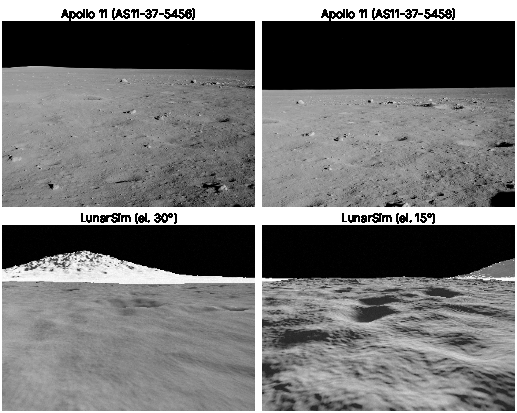
\includegraphics[width=\columnwidth]{figures/apollo_vs_sim.pdf}
\caption{Real Apollo~11 surface photographs~\cite{apollo11} (top) and LunarSim renders (bottom).
The renderer reproduces the black sky, the horizon structure and the shading statistics of
low-Sun regolith. It under-resolves near-field rocks smaller than the $0.3$\,m DEM spacing, a
limitation discussed in \cref{sec:limits}.}
\label{fig:apollo}
\end{figure}

\paragraph*{Photometry and shadows}
Radiance follows the lunar-Lambert function of McEwen~\cite{mcewen1991photometric},
$I\propto A\,[2L(g)\cos i/(\cos i+\cos e)+(1-L(g))\cos i]$, with phase-dependent $L(g)$. It is
multiplied by a Hapke-style shadow-hiding opposition term
$1+B_0/(1+\tan(g/2)/h)$~\cite{hapke2012theory}, where $i$, $e$ and $g$ are the incidence, emission and
phase angles. Cast shadows are computed from both DEMs (so massifs shade the valley at low Sun),
averaged over the $0.53^\circ$ solar disk to produce penumbrae. A weak ambient term models
earthshine and inter-reflection, and a footprint-faded micro-relief bump map adds sub-grid regolith
texture.

\paragraph*{Camera}
A rover-mounted pinhole camera ($70^\circ$ HFOV, $320\times240$, $1.35$--$1.7$\,m high) is rendered
by column-wise height-field ray casting, accounting for lunar curvature. The renderer applies
centre-weighted auto-exposure, a soft-shoulder tone curve, gamma, shot and read noise, and 8-bit
quantisation. One image takes about $0.15$\,s on a CPU once the shadow maps for a Sun direction
have been computed.

\paragraph*{Protocol}
Each scene contains a smooth random traverse with places every $6$\,m. The database is rendered at
one Sun direction (azimuth $135^\circ$, elevation $30^\circ$). Queries are taken at jittered poses
(up to $3$\,m offset, $\mathcal{N}(0,10^\circ)$ heading noise, random camera height). The
\emph{same} query poses are rendered under seven Sun conditions (\cref{tab:conds}), so differences
between conditions are paired and caused by illumination alone. The test set has three unseen
scenes ($3\times150$ database images and $3\times1050$ queries), the validation set one scene
($100$ places, $700$ queries), and the training set five further scenes with $240$ places $\times$
$4$ views. Training views use Sun directions drawn from a per-scene pool of $16$ random
directions (elevation $4^\circ$--$75^\circ$, any azimuth), which mimics an illumination-sweep
dataset.

\begin{table}[t]
\centering
\caption{Query illumination conditions (Sun azimuth/elevation in degrees). The database is rendered at
azimuth $135^\circ$, elevation $30^\circ$.}
\label{tab:conds}
\scriptsize
\setlength{\tabcolsep}{3pt}
\begin{tabular}{@{}lccccccc@{}}
\toprule
 & C0 & C1 & C2 & C3 & C4 & C5 & C6 \\
\midrule
Az./El. & 135/30 & 135/15 & 135/6 & 135/60 & 225/30 & 315/30 & 315/8 \\
Change & view & lower & grazing & high & rot.\ $90^\circ$ & flip & flip+graz.\ \\
\bottomrule
\end{tabular}
\end{table}

% ======================================================================
\section{Experiments}\label{sec:exp}
% ======================================================================
\subsection{Setup}\label{sec:setup}
\paragraph*{Compared methods}
\emph{Zero-shot terrestrial models} use their official weights: CosPlace-R50~\cite{berton2022cosplace}
($512$-D), EigenPlaces-R50~\cite{berton2023eigenplaces} ($2048$-D) and DINOv2-SALAD~\cite{izquierdo2024optimal}
($8448$-D, trained on GSV-Cities~\cite{alibey2022gsv}). \emph{Lunar-trained heads} all share the
frozen SALAD-fine-tuned DINOv2 ViT-B/14 backbone, the training data, the loss and the schedule, and
differ only in the aggregation: GeM~\cite{radenovic2019gem} ($1280$-D), NetVLAD~\cite{arandjelovic2016netvlad}
($k$-means-initialised, $64\times128$ + scene token, $8448$-D), SALAD (balanced OT, $\lambda=1$) and
Galatea (semi-relaxed UOT with learned $\lambda$). The last three have identical descriptor size
and almost identical parameter counts. For stage~2 we compare four local scorers on the same
SuperPoint keypoints (top $384$ by score) and top-$K=10$ candidates: mutual nearest neighbours
with cosine $>0.7$ (MNN), training-free entropic OT with dust-bins (UOT, appearance only), the learned LightGlue
matcher~\cite{lindenberger2023lightglue}, and our partial FGW. Each is used with and without
MAGSAC++ verification.

\paragraph*{Implementation}
Images are resized to $210\times280$ for the ViT ($n=300$ tokens). Heads are trained with AdamW
(learning rate $4\cdot10^{-4}$, one-cycle schedule, weight decay $10^{-4}$) for $500$ steps of $24$
places $\times$ $4$ views, using the multi-similarity loss ($\alpha=1$, $\beta=50$, miner margin $0.1$).
Sinkhorn uses $L=3$ iterations, $m=64$ clusters and $\ell=128$. The four main heads and the $\lambda=0$ ablation
are run with three seeds (mean $\pm$ standard deviation); the other ablations use one seed. For stage~2, the structural weight $\alpha\in\{0,0.3,0.6\}$ (chosen: $0.3$) and the fusion
parameters $\beta,\kappa$ are selected on the validation scene only. $\varepsilon_\ell=0.05$ and the
dust-bin cost threshold $0.25$ (cosine $0.75$) are fixed a priori, and MAGSAC++ uses a $1.5$\,px threshold. All experiments run on a $2$-core CPU without a GPU. Code, the renderer, the rendered
benchmark and the trained heads are available at \url{https://github.com/RaunakDune/galatea-lunar-vpr}.


\begin{figure*}[t]
\centering
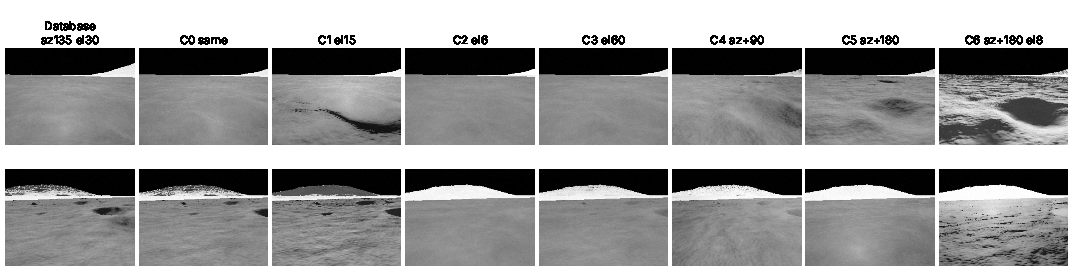
\includegraphics[width=\textwidth]{figures/conditions.pdf}
\caption{LunarSim-VPR: two test places (rows). Left: database image (Sun azimuth $135^\circ$,
elevation $30^\circ$). Right: queries at a jittered pose under the seven Sun conditions of
\cref{tab:conds}. Rendered with lunar-Lambert photometry, opposition surge and cast shadows from
local and regional relief. In the top row at C2, the camera lies in the shadow of a distant massif
and is lit only by the weak ambient term.}
\label{fig:conds}
\end{figure*}
\begin{figure}[t]
\centering
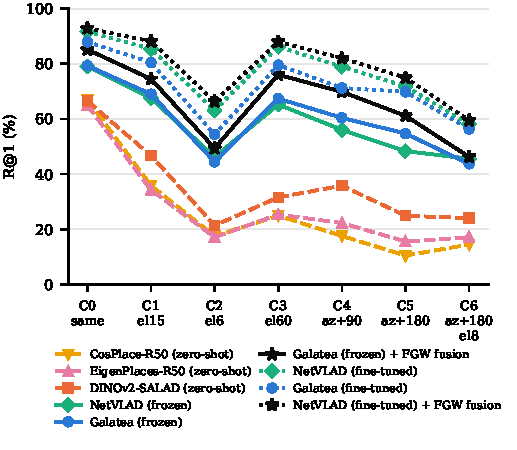
\includegraphics[width=\columnwidth]{figures/percond.pdf}
\caption{R@1 per illumination condition on the test set. Zero-shot terrestrial models (dashed)
collapse once the Sun moves. Lunar-trained OT aggregation (Galatea) and global--local fusion
(Galatea + FGW) recover much of the loss, most of all under shadow reversal and grazing light.}
\label{fig:percond}
\end{figure}

\begin{table*}[t]
\centering
\caption{Recall (\%) on the LunarSim-VPR test set (3 unseen scenes, 3150 queries). Lunar-trained heads share the frozen DINOv2 backbone and training protocol; mean$\pm$std over 3 seeds. Per-condition columns give R@1 (conditions in \cref{tab:conds}).}
\label{tab:main}
\footnotesize
\setlength{\tabcolsep}{4pt}
\begin{tabular}{@{}llr ccc ccccccc@{}}
\toprule
& Method & Dim. & R@1 & R@5 & R@10 & C0 & C1 & C2 & C3 & C4 & C5 & C6 \\
\midrule
\multirow{3}{*}{\rotatebox{90}{\scriptsize zero-shot}} & CosPlace-R50~\cite{berton2022cosplace} & 512 & 26.8 & 50.3 & 60.8 & 66.9 & 35.8 & 17.6 & 24.9 & 17.6 & 10.4 & 14.4 \\
 & EigenPlaces-R50~\cite{berton2023eigenplaces} & 2048 & 28.1 & 53.0 & 64.1 & 64.9 & 34.2 & 17.1 & 25.3 & 22.2 & 15.6 & 17.1 \\
 & DINOv2-SALAD~\cite{izquierdo2024optimal} & 8448 & 35.8 & 65.4 & 77.7 & 66.4 & 46.7 & 21.3 & 31.6 & 35.8 & 24.9 & 24.0 \\
\midrule
\multirow{4}{*}{\rotatebox{90}{\scriptsize lunar-trained}} & GeM & 1280 & 31.5{\scriptsize$\pm$0.4} & 64.7{\scriptsize$\pm$0.3} & 79.4{\scriptsize$\pm$0.2} & 55.0 & 34.8 & 19.8 & 35.3 & 30.1 & 25.1 & 20.3 \\
 & NetVLAD & 8448 & 58.2{\scriptsize$\pm$0.7} & 86.6{\scriptsize$\pm$0.4} & 94.6{\scriptsize$\pm$0.2} & 79.0 & 67.5 & 46.1 & 65.2 & 56.0 & 48.3 & 45.6 \\
 & SALAD ($\lambda{=}1$) & 8448 & 59.4{\scriptsize$\pm$0.7} & \textbf{87.3{\scriptsize$\pm$0.7}} & \textbf{94.8{\scriptsize$\pm$0.2}} & 77.6 & 68.4 & \textbf{46.4} & 65.4 & 58.6 & 52.7 & \textbf{46.7} \\
 & Galatea, learned $\lambda$ & 8448 & \textbf{59.8{\scriptsize$\pm$0.8}} & \textbf{87.3{\scriptsize$\pm$0.5}} & 94.6{\scriptsize$\pm$0.2} & \textbf{79.3} & \textbf{69.0} & 44.4 & \textbf{67.3} & \textbf{60.4} & \textbf{54.7} & 43.7 \\
\bottomrule
\end{tabular}
\end{table*}

\subsection{Terrestrial models under lunar illumination change}\label{sec:zeroshot}
\Cref{tab:main} (top) shows that all three terrestrial models perform reasonably when only the
viewpoint changes: at C0, R@1 is $\zsEigCzero$--$\zsCosCzero\%$. They degrade sharply as soon as the
Sun moves. DINOv2-SALAD, the strongest of them, falls from $\zsSaladCzero\%$ at C0 to
$\zsSaladCtwo\%$ under grazing illumination (C2) and to $\zsSaladCfive\%$ when the shadows flip (C5).
The CNN-based CosPlace and EigenPlaces fare worse, with C5 values of $\zsCosCfive\%$ and $\zsEigCfive\%$.
Even a foundation-model backbone pre-trained on 142M images therefore does not provide
illumination-invariant place descriptors on regolith. Local re-ranking does not close the gap
either. Fusing MNN+MAGSAC++ matches into the top-10 zero-shot SALAD candidates (selected on
validation as in \cref{sec:rerank}) raises R@1 to $\zsRRRone\%$. That is still below the lunar-trained
stage~1 \emph{without} re-ranking, and only $\zsRRHard\%$ on the hardest conditions, because the
correct place is often not among the candidates at all.

\subsection{Lunar-adapted OT aggregation}\label{sec:stage1}
Training only the aggregation head on illumination-diverse LunarSim scenes (backbone frozen) lifts
R@1 from $\zsSaladRone\%$ to $\galRone\%$ (Galatea, mean of three seeds). On the paired test queries
this is a gain of $\gainZsMean$ points (95\% CI $[\gainZsLo,\gainZsHi]$). The largest gains are under
illumination change. Mean R@1 over the three hardest conditions (C2, C5, C6) rises from $\zsSaladHard\%$
to $\galHard\%$. The three cluster-based heads (NetVLAD, SALAD and Galatea) clearly beat every zero-shot model.
GeM pooling of the same frozen tokens does not ($\gemRone\%$). Without fine-tuning the backbone,
global pooling cannot separate place-specific tokens from illumination-dependent ones, while
cluster-based aggregation can~\cite{izquierdo2024optimal}.

Galatea and SALAD are statistically indistinguishable: the paired difference in R@1 is
$\galVsSalMean$ points (95\% CI $[\galVsSalLo,\galVsSalHi]$), as \cref{prop:colinv} predicts. The two heads differ sharply in how they spend mass. The balanced head sends
$\salDust\%$ of all token mass to the dust-bin, and its total dust-bin mass correlates with the sky
fraction of the image ($\rho=\salSkyCorr$). The learned unbalanced head ($\bar\lambda=\galLam$)
discards only $\galDust\%$ and concentrates the remaining mass on a few clusters (coefficient of
variation of cluster mass $\galCV$ vs.\ $\salCV$). Their retrieval performance is nevertheless the
same. On this data, therefore, the assignment's marginal constraints are not the bottleneck; the
training distribution is. We return to this in \cref{sec:ablation}.

\begin{table}[t]
\centering
\caption{Stage-2 re-ranking of the top-10 Galatea candidates (test, \%). \emph{Local}: sort by the local score only. \emph{Fused}: \cref{eq:fusion} with $(\beta,\kappa)$ chosen on the validation scene.}
\label{tab:rerank}
\footnotesize
\setlength{\tabcolsep}{3pt}
\begin{tabular}{@{}lcccc@{}}
\toprule
& \multicolumn{2}{c}{Local} & \multicolumn{2}{c}{Fused} \\
\cmidrule(lr){2-3}\cmidrule(lr){4-5}
Local scorer & R@1 & R@5 & R@1 & R@5 \\
\midrule
none (global ranking) & \multicolumn{2}{c}{--} & 60.8 & 88.0 \\
MNN & 59.2 & 88.2 & 66.0 & 89.5 \\
MNN + MAGSAC++ & 62.4 & 89.2 & \textbf{67.2} & 90.0 \\
OT, appearance only & 57.0 & 89.5 & 65.8 & 90.4 \\
OT, appearance only + MAGSAC++ & 61.0 & 88.3 & 63.0 & 88.6 \\
LightGlue~\cite{lindenberger2023lightglue} (learned) & 57.5 & 87.4 & 65.3 & 89.6 \\
LightGlue~\cite{lindenberger2023lightglue} (learned) + MAGSAC++ & 60.0 & 89.0 & 65.7 & 89.8 \\
Partial FGW (ours) & 59.8 & 90.1 & 66.0 & 90.1 \\
Partial FGW (ours) + MAGSAC++ & 63.0 & 88.6 & 63.8 & 88.7 \\
\bottomrule
\end{tabular}
\end{table}

\subsection{Global--local fusion with OT re-ranking}\label{sec:rerank}
\Cref{tab:rerank} re-ranks the top-10 candidates of Galatea (seed 0, R@1 $\rrGlobRone\%$).
Two findings stand out. First, ranking by the local score alone barely helps and can hurt: no scorer
improves R@1 by more than about two points, and several lose ground. The reason is that SuperPoint
responses on regolith are dominated by shadow edges, which move with the Sun. Second, fusing local
and global evidence with \cref{eq:fusion} helps every scorer. With partial FGW, R@1 rises to
$\rrFgwRone\%$, a gain of $\rrGainMean$ points (95\% CI $[\rrGainLo,\rrGainHi]$), and on the hardest
conditions from $\galSzeroHard\%$ to $\rrFgwHard\%$, the best of all scorers on that subset.
Differences between scorers in the fused setting are small and within the confidence intervals:
FGW vs.\ LightGlue $\fgwVsLgMean$ $[\fgwVsLgLo,\fgwVsLgHi]$, and FGW vs.\ appearance-only OT
$\fgwVsUotMean$ $[\fgwVsUotLo,\fgwVsUotHi]$. The training-free structural matcher thus performs as
well as a learned terrestrial matcher. MAGSAC++ helps MNN and LightGlue but not the OT matchers, whose dust-bins already reject outliers.
The effect is robust across stage-1 seeds. Repeating the protocol on all three Galatea seeds
(re-tuning $\beta,\kappa$ on validation each time), fusion gains $\msFgwGain\pm\msFgwGainsd$ points R@1
with FGW, $\msMnnRGain\pm\msMnnRGainsd$ with MNN+MAGSAC++ and $\msMnnGain\pm\msMnnGainsd$ with plain MNN.
The practical lesson is that, on the Moon, \emph{how local and global evidence are combined matters
more than which local matcher is used}.

\begin{table}[t]
\centering
\caption{Ablations of the stage-1 aggregator (test R@1/R@5, \%; hard = mean R@1 over C2, C5, C6). Top: assignment relaxation $\lambda$ (mean$\pm$std over the seeds available; single-seed rows marked $^\dagger$). Bottom: Galatea variants vs.\ the seed-0 reference.}
\label{tab:ablation}
\footnotesize
\setlength{\tabcolsep}{3.5pt}
\begin{tabular}{@{}lccc@{}}
\toprule
Variant & R@1 & R@5 & hard \\
\midrule
$\lambda=0$ (NetVLAD assignment + dust-bin) & 59.9{\scriptsize$\pm$0.8} & 87.6{\scriptsize$\pm$0.6} & 48.4 \\
$\lambda=0.25$ (fixed)$^\dagger$ & 60.7 & 88.2 & 48.1 \\
$\lambda$ learned (Galatea, init.\ 0.5) ($\bar\lambda{=}0.50$) & 59.8{\scriptsize$\pm$0.8} & 87.3{\scriptsize$\pm$0.5} & 47.6 \\
$\lambda$ learned, $25\times$ lr on $\lambda,z$ ($\bar\lambda{=}0.56$)$^\dagger$ & 60.3 & 87.7 & 47.3 \\
$\lambda=0.75$ (fixed)$^\dagger$ & 59.2 & 87.9 & 48.2 \\
$\lambda=1$ (SALAD, balanced) & 59.4{\scriptsize$\pm$0.7} & 87.3{\scriptsize$\pm$0.7} & 48.6 \\
\midrule
Galatea (seed 0, reference) & 60.8 & 88.0 & 47.8 \\
\quad no dust-bin & 62.1 & 88.0 & 49.3 \\
\quad $L=1$ Sinkhorn iteration & 59.9 & 87.8 & 46.6 \\
\quad $L=10$ iterations & 60.7 & 88.0 & 47.7 \\
\quad $m=16$ clusters & 57.7 & 86.2 & 45.9 \\
\quad $m=32$ clusters & 61.1 & 88.2 & 47.9 \\
\quad single-illumination training & 47.3 & 72.2 & 27.6 \\
\bottomrule
\end{tabular}
\end{table}

\subsection{Ablations}\label{sec:ablation}
\Cref{tab:ablation} varies one factor at a time on seed~0. Single-seed differences below about two
points should be read against the seed standard deviation of roughly one point (\cref{tab:main}).

\paragraph*{Illumination-diverse training}
Re-rendering the five training scenes with the \emph{same} poses but a single Sun direction (that of
the database) has by far the largest effect of any factor we varied. The frozen Galatea head then
reaches only $\fixIllRone\%$ R@1, $\fixIllDrop$ points below illumination-diverse training, and SALAD
drops the same way ($\salFixIllRone\%$). The single-illumination model is slightly \emph{better} when
the query light matches its training light (C0: $\fixIllCzero\%$ vs.\ $\galSzeroCzero\%$), but on the
three hardest conditions it falls to $\fixIllHardVal\%$, against $\galSzeroHard\%$. Fine-tuning makes
this worse, not better: with a single training Sun the fine-tuned Galatea reaches $\ftFixIllRone\%$
($-\ftFixIllDrop$ points; C0 $\ftFixIllCzero\%$ vs.\ $\ftGalSzeroCzero\%$, hard $\ftFixIllHard\%$ vs.\
$\ftGalSzeroHard\%$) and SALAD $\ftSalFixIllRone\%$. A more flexible model fits the training light more
closely, so backbone adaptation is only useful together with illumination diversity. For lunar VPR,
an illumination sweep in the training data, as provided by renderers such as LunarSim or DEM-based
pipelines, matters far more than the choice of aggregation layer.

\paragraph*{Sinkhorn iterations and clusters}
Changing the number of Sinkhorn iterations ($L=1$: $\LoneRone\%$, $L=10$: $\LtenRone\%$) moves R@1 by
less than seed noise, in line with prediction (P3) and the fast contraction of
\cref{prop:contraction}. Halving the clusters to $m=32$ ($4352$-D) costs nothing
($\mThirtytwoRone\%$), which is attractive for bandwidth-limited rovers. With $m=16$ ($2304$-D), R@1
drops to $\mSixteenRone\%$.


\subsection{Run time}\label{sec:runtime}
On the same 2-core CPU, the frozen ViT-B/14 takes $\tBackbone$\,ms per image and SuperPoint
$\tSp$\,ms. The heads add only $\tNv$--$\tGal$\,ms (Galatea: $\tGal$\,ms), so the $\lambda$-scaled
Sinkhorn loop is negligible. Per candidate pair (200 keypoints), appearance-only OT takes
$\tUot$\,ms, LightGlue $\tLg$\,ms and partial FGW $\tFgw$\,ms. FGW re-ranking of $K=10$ candidates
thus costs about $\tFgwK$\,ms per query, so MNN+MAGSAC++ is the cheaper choice at similar accuracy.


\ifrealdata
\subsection{Real lunar imagery}\label{sec:real}
% AUTHOR: insert the re-run Despina / Apollo evaluation here (Recall@1/5/10, same protocol).
\fi

\subsection{Limitations}\label{sec:limits}
All quantitative results come from simulation. LunarSim reproduces the statistical character of
lunar relief and the dominant photometric effects, but it omits several things: resolved near-field rocks below the $0.3$\,m DEM spacing (\cref{fig:apollo}), multiple
scattering beyond a constant ambient term, rover self-shadowing and dust, lens flare, exposure
bracketing, and the full range of geological units. Absolute recall values should therefore not be
read as predictions of on-Moon performance. The \emph{relative} comparisons are made under
identical conditions and with paired queries. Because the backbone is frozen and no method sees
test scenes, we expect these comparisons to carry over better than the absolute values, but this
must be confirmed on real imagery. The backbone was frozen because of compute constraints, and
joint fine-tuning may change the ranking between heads. The FGW structural term uses image-plane
distances, which are only approximately preserved under large viewpoint changes. Lifting database
keypoints to 3-D with DEM depth is a natural extension.

% ======================================================================
\section{Conclusion}\label{sec:conclusion}
% ======================================================================
Galatea treats both stages of lunar place recognition as optimal-transport problems. For
aggregation, a semi-relaxed unbalanced formulation unifies the NetVLAD and SALAD assignments under
one parameter. It comes with an explicit convergence rate, a closed-form view of the dust-bin, and
an invariance result showing that intra-normalised descriptors see the plan only through token
weights. For re-ranking, partial fused Gromov--Wasserstein matching adds the relative layout of
keypoints to their appearance, and a saturating fusion merges local and global evidence. On the
LunarSim-VPR benchmark, three findings are useful for practitioners:
(i)~terrestrial models, including foundation-model ones, lose more than half their recall under
large Sun changes;
(ii)~illumination-diverse training data is worth far more than the choice of aggregation layer,
and, as predicted by the theory, balanced and unbalanced assignments perform alike;
(iii)~fusing local with global evidence adds five to seven points of Recall@1 regardless of the
local matcher, whereas re-ranking by local evidence alone helps little.
The next steps are evaluation on DEM-registered real imagery, joint fine-tuning of the backbone,
and 3-D structural terms that use the database's DEM depth.



\bibliographystyle{IEEEtran}
\bibliography{refs}

% Proofs are provided in the supplementary material (supplement.tex) to respect the RA-L page limit.

\end{document}
